\documentclass[oneside]{article}

% Language setting
% Replace `english' with e.g. `spanish' to change the document language
\usepackage[english]{babel}
\usepackage[utf8]{inputenc} % für Umlaute
\usepackage{fontenc}

% Set page size and margins
% Replace `letterpaper' with`a4paper' for UK/EU standard size
\usepackage[a4paper,top=2cm,bottom=2cm,left=3cm,right=3cm,marginparwidth=1.75cm]{geometry}

%%%% ---- Useful packages

%%% --- Colors
\usepackage[dvipsnames]{xcolor}

%%% --- Figures and Graphics
\usepackage{graphicx}
\usepackage{subcaption}
\usepackage{tikz}

%%% --- Tabulars
\usepackage{booktabs}
\usepackage{multirow} % cells over several rows
\usepackage{tabularx}
\usepackage{tabularray}

%%% --- Mathematics
\usepackage{amsmath,amsfonts,amssymb,amsthm,mathtools, mathabx}
\usepackage{bm} % bold mathematics
\usepackage{bbm} % for blackboard 1
\usepackage[linesnumbered,lined,algo2e,figure,boxed]{algorithm2e}
\usepackage[short]{optidef} % for aligning linear programs

%%% --- Other
\usepackage[colorlinks=true, allcolors=blue]{hyperref}
%\usepackage[hidelinks]{hyperref}
\usepackage[style=authoryear,backend=bibtex]{biblatex}
\addbibresource{library.bib}
\usepackage{csquotes}
\usepackage[shortcuts]{extdash} % For Hyphens in English
%\usepackage{acro}
% \DeclareAcronym{pdf}{short=PDF, long={probability distribution function}}

%%% --- Commenting, Todonotes
\usepackage[colorinlistoftodos,prependcaption]{todonotes}
\usepackage{comment, soul}
\newcommand{\ar}{$\rightarrow$}
\presetkeys{todonotes}{backgroundcolor=yellow!30, bordercolor=yellow!50, linecolor=yellow!50, figwidth=\textwidth}{}
%\newcommand{\hl}[1]{\textcolor{Aquamarine}{#1}}

\usepackage{xargs} % Use optional arguements in commands
\newcommandx{\unsure}[2][1=]{\todo[linecolor=blue,backgroundcolor=blue!25,bordercolor=blue,#1]{#2}}
\newcommandx{\missing}[2][1=]{\todo[linecolor=red,backgroundcolor=red!25,bordercolor=red,#1]{#2}}
\newcommandx{\change}[2][1=]{\todo[linecolor=red,backgroundcolor=red!25,bordercolor=red,#1]{#2}}
\newcommandx{\info}[2][1=]{\todo[linecolor=OliveGreen,backgroundcolor=OliveGreen!25,bordercolor=OliveGreen,#1]{#2}}
\newcommandx{\improvement}[2][1=]{\todo[linecolor=Plum,backgroundcolor=Plum!25,bordercolor=Plum,#1]{#2}}
\newcommandx{\thiswillnotshow}[2][1=]{\todo[disable,#1]{#2}}
\usepackage{marginnote}
\let\marginpar\marginnote

%%%% ---- Own Commands
%%% --- Theorem Settings
\theoremstyle{plain}% Theorem-like structures provided by amsthm.sty
\newtheorem{theorem}{Theorem}
\newtheorem{exa}{Example}
\newtheorem{rem}{Remark}
\newtheorem{proposition}{Proposition}
\newtheorem{lemma}{Lemma}
\newtheorem{corollary}{Corollary}

\theoremstyle{definition}
\newtheorem{definition}{Definition}
\newtheorem{remark}{Remark}
\newtheorem{example}{Example}

%%% --- Math Commands

\newcommand{\lag}[1][l]{\Delta_{#1}}
\DeclarePairedDelimiter{\abs}\lvert\rvert
\DeclareMathOperator{\sign}{sign}
\newcommand{\tmax}{\bar{t}}
\newcommand{\ind}[1]{\mathbbm{1}\{#1\}}
\newcommand{\ydiff}{D y}
\newcommand{\ydifft}{Dy^\star}
\newcommand{\xdiff}{Dx}
\newcommand{\xdifft}{Dx^\star}
\newcommand{\Ydiff}{DY}
\newcommand{\Xdiff}{DX}
\newcommand{\Prob}[1]{P(#1)}
\newcommand{\mprob}{\tilde{m}}
\newcommand{\Ber}{\text{Ber}}
\newcommand{\SBer}{\text{SBer}}
\newcommand{\cond}{\:\lvert\:}

%%% --- Other Commands
\renewcommand{\arraystretch}{1.2}

%%% --- ToDo List
\usepackage{enumitem}
\newlist{todolist}{itemize}{2}
\setlist[todolist]{label=$\square$}
\usepackage{pifont}
\newcommand{\cmark}{\ding{51}}%
\newcommand{\xmark}{\ding{55}}%
\newcommand{\done}{\rlap{$\square$}{\raisebox{2pt}{\large\hspace{1pt}\cmark}}%
\hspace{-2.5pt}}
\newcommand{\wontfix}{\rlap{$\square$}{\large\hspace{1pt}\xmark}}

\title{Assessment and Optimization of Nowcast Measures for Trend Detection}
\author{Oliver Grothe, Bolin Liu, Jonas Rieger}

\begin{document}
\maketitle

\begin{abstract}
Existing and new measures for the capability of capturing the trend of nowcasts are presented, evaluated, and compared on synthetic and real-world data.
\end{abstract}

\subsection*{Offene Punkte}

\begin{itemize}
    \item Welche Form sollte das Maß haben? Mögliche Wahlen: Indikator, Probabilistisch, verschiedene Gewichtungen, ... (Siehe Tabelle \ref{tab:comparison-measures})
    \item Indikator oder Signum?
    \item Schätzung/Wahl des Rauschparameters $\sigma$ bei Maßen außer Indikator
    \item Gehen wir auf andere Verteilungen für den Fehler ein?
    \item Konfidenzintervalle
\end{itemize}

\listoftodos


\section{Introduction}

\begin{itemize}
	\item Trending is an important feature of nowcasts to be identify changes in the situation before the actual quantity can be measured
	\item What scores are currently used?
	\item Examples: Covid, BIP, Medicine, ... 
 \item Nice an comprehensive introduction to nowcasting, so that it becomes clear for non-nowcasters what is special about nowcasting
 \item Measurements and Forecasting; What are the differences to nowcasting from a modeling point of view?
\end{itemize}


\section{Trend measures for nowcasts}

Notation
\begin{itemize}
  \item Let $y_1, \ldots, y_T$ be the values of the nowcasted quantity.
  \item Let $x_t^k$ be the $k$-th nowcast for time $t = 1, \ldots, T$ (possibly after some aggregation if several raw nowcasts apply).
  \item Let $\ydiff_t = y_t - y_{t-1}$ be the change that occurred between the time steps $t-1$ and $t$ and $\xdiff_t^k = x_t - \mathcal{x}_{t-1}$ the change nowcaster $k$ issued between the time steps. Let us first assume that $y_{t-1}$ is available at time $t$ so that it can be used for the evaluation. 
  In Section \hl{error-model-section}, we expand on other reasonable choices for $\mathcal{x}_{t-1}$.
  \item Then, $\xdiff_t^k$ can be seen as the point forecast of nowcaster $k$ for $\ydiff_t$. 
\end{itemize}

\subsection{What is the trend of a nowcast?}

Trend: Issuing the right \enquote{direction} of change between two time steps; statistical consistency of $\sign(\ydiff_t)$ and $\sign(\xdiff_t)$ (Problem: mit kleinen Fehlern; Hinweis Exclusion area)

\begin{itemize}
  \item Translate into mathematical notation
  \item Illustrative Example: Two nowcasts of quantity of interest, where one jumps up and down and one points in right direction with the same rmse; small subset of Simulation~\ref{sec:simulation_rmse_mae}; Plot time series \& time series of differences
\end{itemize}

\subsection{Graphical methods}


\begin{itemize}
  \item 4Q-Plot
  \item Andere Medizin-Plots mit Verweis auf Grothe-Paper
\end{itemize}


\subsection{Measures}

Comparsion and outline of various ideas for measures; overview in Table~\ref{tab:comparison-measures}:
\begin{itemize}
    \item Subsection~\ref{sec:equal-weight} Equal-weighted indicator
    \item Subsection~\ref{subsec:w1} Weighted formula by explanatory power of points
    \item Subsection~\ref{subsec:w2} Combined assessment of trend and its estimation uncertainty with weighting by explanatory power of points
    \item A comparison of the Measures of Subsection~\ref{subsec:w1} and Subsection~\ref{subsec:w2} is given in \ref{subsec:w1-w2}
    \item Subsection~\ref{subsec:probabilistic} Probabilistic version of estimation (as historic version)
\end{itemize}

Requirements for a reasonable measure:
\begin{itemize}
    \item $\ydiff = \xdiff$: trending measure should be 1
    \item $\ydiff = - \xdiff$: trending measure should be 0 or -1
    \item Points \enquote{close} to the axis should be treated differently than points that are far away from axis
    \item Scalar multiplication of $y$ or $x$ should not change the trending measure (?)
\end{itemize}

%\begin{table}
%	\centering
%	\begin{tabular}{l l c c}
%	\toprule
%	& & \multicolumn{2}{c}{Observed trend} \\
%	& & $\ydiff_t > 0$ & $\ydiff_t < 0$ \\	\cline{3-4}
%	\multirow{2}{*}{Forecasted trend} & $\xdiff_t > 0$ & hit & false alarm\\
%	& $\xdiff_t < 0$ & miss & correct negative \\
%	\bottomrule
%\end{tabular}
%\end{table}

\begin{table}[]
    \centering
    \begin{tabular}{l l p{4cm} p{4cm} p{4cm}}
    \toprule
    name & abbr. & accuracy & + & - \\ \midrule
    indicator & i & $\frac{1}{T-1} \sum \ind{x_t y_t > 0}$ &  well-known, intuitive & what about points near (0,0) \\
    Probabilistic & p & $\frac{1}{T-1} \sum P{(x_t y_t > 0)}$ & small variance, weighting due to probabilities & unintuitive, asymptotics unclear, driven towards 0.5, no standard estimation for $\sigma$  \\
    weighted 1 (*) & w1 & {\small {$\sum w_i \ind{x_t y_t > 0} / \sum w_i$,\newline $w_i = \max_j\{P(y_i, x_i) \in Q_j \} - 0.25$}} & intuitive, natural extension, implicit exclusion area as points near (0,0) do not gain weight & \\ \bottomrule
    \end{tabular}
    \caption{Comparison between different measures for accuracy. For the weighted measures, the indicator could be replaced by the signum function of the product.}
    \label{tab:comparison-measures}
\end{table}

\subsubsection{Equal-weighted indicators} \label{sec:equal-weight}

Natural evaluation method for 4Q-plot, as known from dichotomous event evaluation, evaluation of classification (confusion matrix):

\begin{tabularx}{\textwidth}{p{5cm} X}
     Accuracy & $m_{\text{acc}} = \frac{\sum_{t=T-w}^T \ind{\ydiff_t > 0, \xdiff_t > 0} + \sum_{t=T-w}^T \ind{\ydiff_t < 0, \xdiff_t < 0}}{T-w}$ \\
     Capability of detecting a positive trend (probability of detection)/Sensitivity & $m_{\text{py}} = \frac{\sum_{t=T-w}^T \ind{\ydiff_t > 0, \xdiff_t > 0}}{\sum_{t=T-w}^T \ind{\ydiff_t > 0}}$ \\
     Positive predictive values & $ m_{\text{px}} = \frac{\sum_{t=T-w}^T \ind{\ydiff_t > 0, \xdiff_t > 0}}{\sum_{t=T-w}^T \ind{\xdiff_t > 0}}$ \\
     Specificity & $m_{\text{ny}} =  \frac{\sum_{t=T-w}^T \ind{\ydiff_t < 0, \xdiff_t < 0}}{\sum_{t=T-w}^T \ind{\ydiff_t < 0}} $ \\
     Negative predictive value & $m_{\text{nx}} =  \frac{\sum_{t=T-w}^T \ind{\ydiff_t < 0, \xdiff_t < 0}}{\sum_{t=T-w}^T \ind{\xdiff_t < 0}}$
\end{tabularx}

Different setting here: We do not only have binary predictions and realization, but we do know the real values behind; intuitive evaluation of a 4Q-plot assigns a greater explanatory power to point far away from (0,0), as small deviations from (0,0) could be driven by noise.



% Extension 1: 
% \begin{itemize}
%   \item 
% Adapt the measures to be weighted by the explanatory power of the points:\\
% Weights $\omega_t$ for $(\ydiff_t, \xdiff_t)$ could be determined by error model and corresponds to the maximal likeliness of the point belonging to the different quadrants ($Q_1, \dots, Q_4$); thus, point that have less explanatory power for assessing the trending ability becomes less weight:
%  	\begin{equation}
%   		\omega_t = \max_{i \in [4]} {P\big( (\ydifft_t, \xdifft_t) \in Q_i \cond \ydiff_t, \xdiff_t \big)} 
% 	\end{equation}
% 	\item E.g., the accuracy becomes
% 	\begin{equation}
%   m_{acc, \omega} = \frac{\sum_{t=T-w}^T \omega_t \ind{\ydiff_t \cdot \xdiff_t > 0} }{\sum_{t=T-w}^T \omega_t}
% \end{equation}
% 	\item Thus, $\omega_t \in [0.25, 1]$. Maybe it would make sense to \enquote{ignore} values without explanatory power and use $\omega_t^\star = 4/3 \ \omega_t \in [0, 1]$ \hl{w2}
% 	\item Figure~\ref{fig:comparison_estimators} shows the resulting estimates for the simulation study comparing the pure indicator, the probability-version and the weighted indicator estimation; the data is generated (in a very simpel model) by
% 	\begin{align}
% 		\ydifft_t &\sim N(0, 2) \\
% 		\xdifft_t &= (2 b_t - 1) \cdot \ydiff_t , b_t \sim \Ber (k) \\
% 		\ydiff_t &= \ydifft_t + \varepsilon_t^y, \varepsilon_t^y \sim N(0, 0.1) \\
% 		\xdiff_t &= \xdifft_t + \varepsilon_t^x, \varepsilon_t^x \sim N(0, 0.1) \\
% 	\end{align}
% \end{itemize}

% \begin{figure}
%   \centering
% 	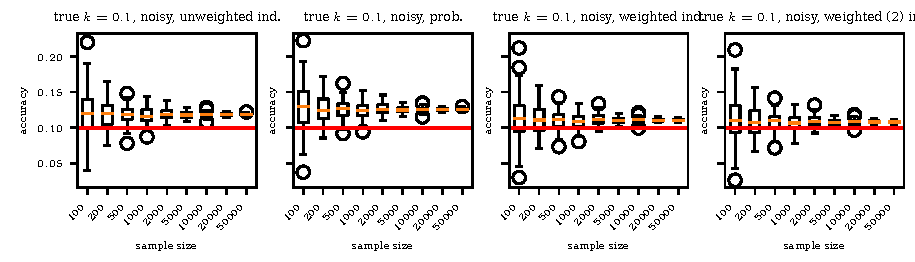
\includegraphics{plots/unbiasedness/boxplot_k_0.1.pdf}
% 	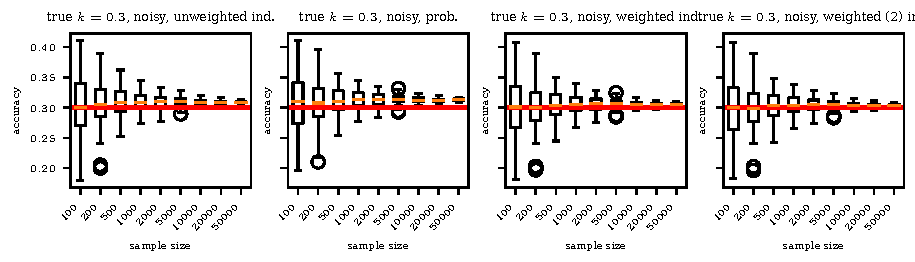
\includegraphics{plots/unbiasedness/boxplot_k_0.3.pdf}
% 	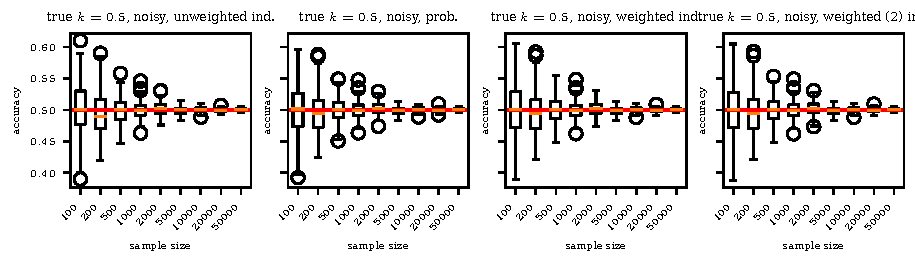
\includegraphics{plots/unbiasedness/boxplot_k_0.5.pdf}
% 	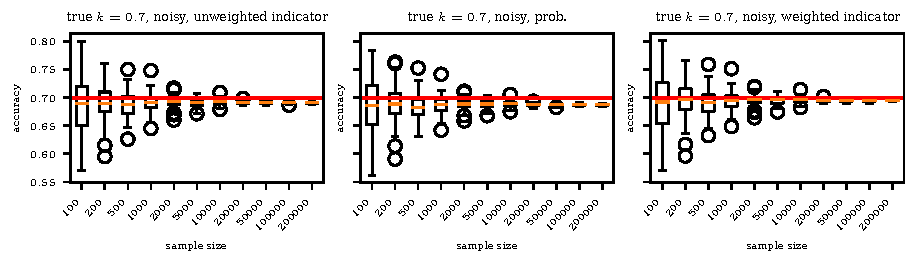
\includegraphics{plots/unbiasedness/boxplot_k_0.7.pdf}
% 	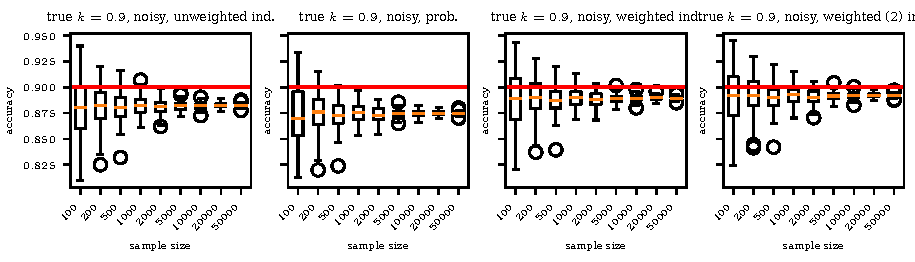
\includegraphics{plots/unbiasedness/boxplot_k_0.9.pdf}			
%   \caption{Simulations results comparing the three types of estimators for the accuracy in a trending setting}
%   \label{fig:comparison_estimators}
% \end{figure}


\subsubsection{Weighted measure by accounting for explanatory power of the points}\label{subsec:w1}

Unlike the situation in dichotomous forecast evaluation or binary classification, the points $(\ydiff_t, \xdiff_t)$ are not binary.
For points with small $\ydiff_t$ and $\xdiff_t$, the sign of their product is more likely to be driven by noise or a nonsystematic relationship.
Weighting the observations by their likelihood to be driven by noise makes the estimation more robust and prevents a decrease of the trending ability because of periods of small and nonsystematic changes. 
A simple method to account for the uncertainty in the measurement of $\ydiff_t$ and $\xdiff_t$ is to assume that the true values $\ydifft_t$ and $\xdifft$ follow (independent) Gaussian distributions around their observed counterparts with standard deviation $\sigma_y$ and $\sigma_y$, respectively.
Then, the estimation can be weighted by how clearly a point can be assigned to one of the quadrants:
\begin{equation}
    m_{\text{acc}}^1 = \frac{\sum_{t=T-w}^T \omega_t \ind{\ydiff_t \xdiff_t > 0} }{\sum w_t}
\end{equation}
with $w_t = \max_{i \in [4]} P((\ydiff_t \xdiff_t) \in Q_i) - 0.25$.
Thus, the $w_t$ are in $[0, 0.75]$ and points very close to $(0, 0)$ do not have any weight in assessing the trend. 
Due to the typical weight structure, $m_{\text{acc}}^1$ is in $[0,1]$ and the bounds are attained if and only if all points are concordant or disconcordant, respectively.

Instead of using the indicator of concordance, one could also use the signum function of the product of $(\ydiff_t, \xdiff_t)$ to scale the result to $(-1, 1)$.
Consistency to the accuracy measure from binary forecasting or classification argues for the indicator function.
Similarly, the weights could be determined as the maximum probability of the true observation lying in $Q_1 \cup Q_3$ or $Q_2 \cup Q_4$.

The estimation uncertainty of $m_{\text{acc}}^1$ can be determined by computing the confidence intervals of the estimation using bootstrapping or by resampling using the Gaussian distribution assumption.

\subsubsection{Combined measure of trending and its uncertainty} \label{subsec:w2}
The points $(Dx_t, Dy_t)$, which are close to the decision boundaries (origin and coordinate axes), should only be of limited informative value for the calculation of the trending measure, as it is uncertain whether such points really belong to the associated quadrants (1,3 or 2,4).

The certainty of belonging can be introduced as a weighting in the indicator formula. The simplest assumption is that the true value of an observed pair of values $(Dx_t,Dy_t)$ is subject to a normal distribution described by the centre $(Dx_t,Dy_t)$ and the covariance 
$\begin{pmatrix} \sigma_x & 0 \\
0 & \sigma_y 
\end{pmatrix}$.

The weights as certainty of affiliation can be calculated as follows:
\[ 
w_t = 
\begin{cases} 
  P(Dx_t \cdot Dy_t > 0) = \left(1 - \Phi\left(\frac{-Dx_t}{\sigma_X}\right)\right)\left(1 - \Phi\left(\frac{-Dy_t}{\sigma_Y}\right)\right) + \Phi\left(\frac{-Dx_t}{\sigma_X}\right) \Phi\left(\frac{-Dy_t}{\sigma_Y}\right) & \text{wenn } Dx_t \cdot Dy_t > 0,  \\
  P(Dx_t \cdot Dy_t < 0) = \left(1 - \Phi\left(\frac{-Dx_t}{\sigma_X}\right)\right) \Phi\left(\frac{-Dy_t}{\sigma_Y}\right) + \Phi\left(\frac{-Dx_t}{\sigma_X}\right) \left(1 - \Phi\left(\frac{-Dy_t}{\sigma_Y}\right)\right)  & \text{wenn } Dx_t \cdot Dy_t < 0,  \\
  0 & \text{sonst} 
\end{cases}
\]

This enables a canonical extension of the indicator formula:


\[m_{\text{acc}} = \frac{\sum_{t=T-w}^T \omega_t \cdot \text{sgn}(Dx_t\cdot Dy_t)}{T-w}\]\\\\
Other normalisation factor: e.g. $\sum_t w_t$ possible, but the following problem: If all points lie in the first quadrant, for example, then the normalisation factor $\sum_t w_t$ always causes the measure $1$, which in some cases does not correspond to intuition, e.g. if the points lie close to the decision limit (in this case one would intuitively expect a slightly positive number). 

Determination of the uncertainty: $\sigma_x$ and $\sigma_y$ reflect the estimate of the uncertainty, i.e. how "far" the true point can be from the observed point in the four-quadrant plot. It is difficult to determine the standard deviations from the data, as the observable data do not contain this information. One empirical method, for example, is to take the empirical variance of $Dx$ and $Dy$ as a reference and calculate values from it (e.g. 10 $\%$ of the variance of $Dx$ and $Dy$).\\\\
Another possibility is to look at the function $(\sigma_x,\sigma_y)\mapsto m_{\text{acc}}(\sigma_x,\sigma_y)$ and make a robust statement (e.g. by optimisation).

\begin{itemize}
    \item Maximum of the function: How much trending is maximally possible taking into account the uncertainty.
    \item Minimum of the function: What is the minimum possible trend taking into account the uncertainty.
    \item Expected value: An additional assumption about the distribution of the uncertainty can be made here, or the mean value of the measures resulting from different $\sigma_x$ and $\sigma_y$ can be calculated for a sufficiently large range of $\sigma_x$ and $\sigma_y$.
\end{itemize}

\newpage
\subsubsection{Comparison of weighted measures using examples} \label{subsec:w1-w2}

Compare the resulting trending assessments for the indicator formula and the weighted schemes. The horizontal axis displays $\ydiff$; the vertical axis corresponds to $\xdiff$. 
The plots show 200 points, but the estimations are computed on 10,000 points.

\noindent
\begin{tblr}{
  colspec = {Q[h]X[-1,m]X[-1,m]X[-1,m]|X[m]},
  width=\textwidth,
  stretch = 0,
  rowsep = 6pt,
}
     & Indicator & Weighted 1 & Weighted 2 & Remarks \\
     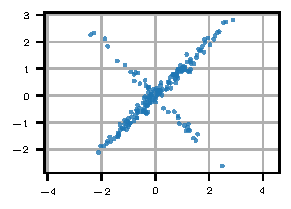
\includegraphics{plots/simulation_comparison_weighted_measures/simple.pdf} & 0.7672 & 0.7836 & 0.7694 &  \\
     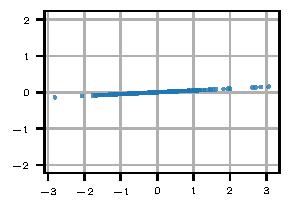
\includegraphics{plots/simulation_comparison_weighted_measures/concordant_no_noise.pdf} & 1 & 1 & 0.8235 & {\scriptsize$\xdiff = \xdifft = 0.05 \ydifft = 0.05 \ydiff$}\newline critique on w1: slight deviation of $\xdiff$ from 0 (near decision boundary), nevertheless, full trending ability. \\
     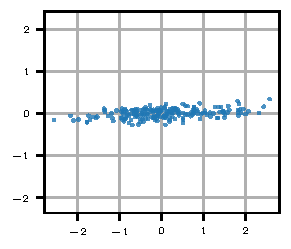
\includegraphics{plots/simulation_comparison_weighted_measures/concordant_noise.pdf} & 0.6466 & 0.6823 & 0.6266 & \\
     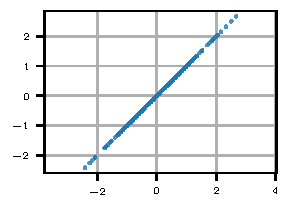
\includegraphics{plots/simulation_comparison_weighted_measures/perfect_normal.pdf} & 1 & 1 & 0.9779 & critique on w2: $\xdiff = \ydiff$, but not trending ability 1\\
    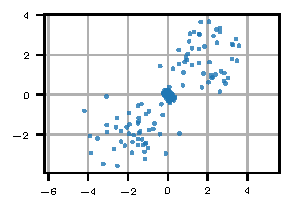
\includegraphics{plots/simulation_comparison_weighted_measures/sure_unsure_combination.pdf} & 0.6152 & 0.6932 & 0.6389 & \\
\end{tblr}


\newpage
\subsubsection{Probabilistic measure (wrong derivation)} \label{subsec:probabilistic}

\improvement[inline]{Due to the additive structure, $(Dx,Dy)$ and $(Dx^*,Dy^*)$ are not independet, and $P(Dy^*\cdot Dx^* > 0|Dx=Dx_t, Dy=Dy_t) $ is difficult to compute}

\begin{itemize}
\item Probabilistic versions of non-probabilistic measures; small sample characteristic of $m_{acc}$ can be driven by random effects near the axis; therefore probabilistic \enquote{correction}:
\begin{itemize}
  \item Assume an additive error decomposition for both observation and nowcast to account for non-systematic and short-term (i.e., intra-day) effects or for effects on inaccurate representation of $y_{t-1}$ in the computation of $Dx_t$ (\hl{this, no additional complexity}):
  	\begin{align}\label{additive error decomposition}
  		\ydiff_t + \varepsilon_t^y &= \ydifft  \\
  		\xdiff_t + \varepsilon_t^x &= \xdifft 
	\end{align}
\item  Replace indicators in the above formulations by the corresponding probabilities:
\begin{align}
		\mprob_{\text{acc}} &= \frac{\sum_{t=T-w}^T \Prob{ \ydifft_t > 0, \xdifft_t > 0} + \sum_{t=T-w}^T \Prob{\ydifft_t < 0, \xdifft_t < 0}}{T-w}  \\
   \mprob_{\text{py}} &= \frac{\sum_{t=T-w}^T \Prob{\ydifft_t > 0, \xdifft_t > 0}}{\sum_{t=T-w}^T \Prob{\ydifft_t > 0}} \\
    \mprob_{\text{px}} &= \frac{\sum_{t=T-w}^T \Prob{\ydifft_t > 0, \xdifft_t > 0}}{\sum_{t=T-w}^T \Prob{\xdifft_t > 0}} \\
    \mprob_{\text{ny}} &= \frac{\sum_{t=T-w}^T \Prob{\ydifft_t < 0, \xdifft_t < 0}}{\sum_{t=T-w}^T \Prob{\ydifft_t < 0}} \\
    \mprob_{\text{px}} &= \frac{\sum_{t=T-w}^T \Prob{\ydifft_t < 0, \xdifft_t < 0}}{\sum_{t=T-w}^T \Prob{\xdifft_t < 0}} 
\end{align} 
\item Simple error model:
  \begin{align}
	  \varepsilon_Y \sim N(0, \sigma_Y) \\
	  \varepsilon_X \sim N(0, \sigma_X)
  \end{align}
  yields, e.g.,
  	\begin{equation}
  		\mprob_{\text{acc}} = \frac{1}{T-w} \sum_{t=T-w}^T  \big( 1 - \Phi_{\ydiff_t, \sigma_y}(0) - \Phi_{\xdiff_t, \sigma_x} (0) + 2 \Phi_{\xdiff_t,\sigma_x}( 0)\Phi_{\ydiff_t,\sigma_y}( 0) \big), 
	\end{equation}
	where $\Phi$ denotes a (possibly multivariate) normal distribution
\end{itemize}
\item For $\sigma_x \sigma_y \rightarrow 0$, the probabilistic measures approach the count-based ones
\item For $\sigma_x \sigma_y \rightarrow \infty$, the probabilistic accuracy approaches   0.5 as all probabilities are approximately 0.5
\item Lag-$l$-measures can easily be obtained by using the $D^l$-difference, i.e., $D^l y_t = y_t - y_{t-l}$
\end{itemize}

\subsection{Estimating the standard deviation of white noise}

First, sometimes variance can be determined heuristically directly from domain knowledge. 
However, to determine the standard deviation of white noise using only the time series data, one can basically follow two approaches, time domain approach or frequency domain approach. For the first approach, a model assumption (e.g. ARIMA models) is specified and the residual analysis technique is applied [\cite{chitturi1974distribution}]. 
In the frequency domain approach, the time series are first decomposed using spectral methods such as (discrete) Fourier transformation [\cite{sauer1992noise}] or wavelet transformation [\cite{heil1989continuous,donoho1994ideal,jansen2012noise}]. After reconstructing the time series, the residuals can be formed in order to determine the standard deviation of white noise. For the use of wavelet, it is particularly convenient that the standard deviation of the white noise can be estimated by the standard deviation of the detail coefficients of the last level, e.g., if the wavelet family db1 is used.

For the noisy signal in the form of \ref{eq: simulation},  there are the following results (cf. pic \ref{fig:estimation std})



%\begin{figure}
%  \centering
%    \begin{subfigure}{0.24\textwidth}
%        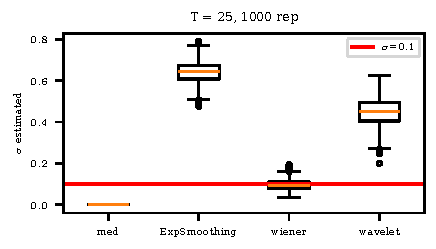
\includegraphics{plots/std estimation/std_estimation_boxplot_25.pdf}
%    \end{subfigure}
%    \begin{subfigure}{0.24\textwidth}
%        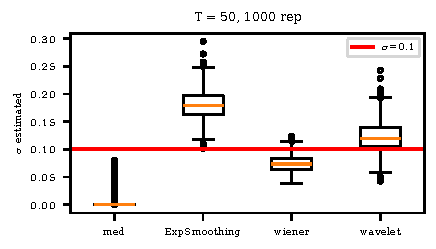
\includegraphics{plots/std estimation/std_estimation_boxplot_50.pdf}
%    \end{subfigure}
%    \begin{subfigure}{0.24\textwidth}
%        \includegraphics{plots/std estimation/std_estimation_boxplot_100.pdf}
%    \end{subfigure}
%    \begin{subfigure}{0.24\textwidth}
%        \includegraphics{plots/std estimation/std_estimation_boxplot_1000.pdf}
%    \end{subfigure}
%  \caption{Estimation of std with different methods.}
%  \label{fig:estimation std}
%\end{figure}%

\begin{figure}
  \centering
    \begin{subfigure}{0.48\textwidth}
        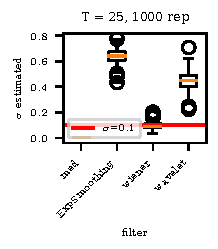
\includegraphics[width=\textwidth]{plots/std_estimation/std_estimation_boxplot_25.pdf}
    \end{subfigure}
    \begin{subfigure}{0.48\textwidth}
        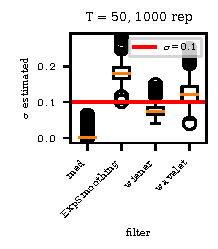
\includegraphics[width=\textwidth]{plots/std_estimation/std_estimation_boxplot_50.pdf}
    \end{subfigure}

    \begin{subfigure}{0.48\textwidth}
        \includegraphics[width=\textwidth]{plots/std_estimation/std_estimation_boxplot_100.pdf}
    \end{subfigure}
    \begin{subfigure}{0.48\textwidth}
        \includegraphics[width=\textwidth]{plots/std_estimation/std_estimation_boxplot_1000.pdf}
    \end{subfigure}

  \caption{Estimation of std using different methods.}
  \label{fig:estimation std}
\end{figure}


\subsection{Confidence intervals and missing data}


\begin{itemize}
  \item Bootstrapping: Compare percentile and BCa approach?
  \item Bootstrapping: What is the \enquote{true} value?
  \item Missing data
\end{itemize}

\subsection{Trending over various time lags}

\begin{itemize}
    \item Introduce plot over several time lags
    \item Question: Re-estimate noise for every lag? 
\end{itemize}


\section{Simulation studies}

\todo{Discuss aims of simulation studies, appropriate study designs and implement}

% \subsection{Bias-Variance tradeoff}

% Simulation:
% \begin{enumerate}
%     \item For $T = 50, 100, 500, 1000$, \verb|dist| in N(0,1), N(0,5), N(0,10), N(1,1), N(1,5), N(1,10), Chi-squared(3), Chi-squared(7), Chi-squared(9)
%     \begin{enumerate}
%         \item For $k \in \{0.05, \dots, 0.95\}$:
%         \begin{enumerate}
%             \item Sample $T$ samples from $\ydifft$ following \verb|dist|
%             \item For $t = 1, \dots, T$: Set $\xdifft_t = \ydifft_t$ with probability $k$, otherwise set $\ydifft_t = - \ydifft_t$
%             \item Set $\ydiff_t = \ydifft + N(0,0.1)$, $\xdiff_t = \xdifft + N(0,0.1)$
%             \item Compute all trending measures
%             \item Repeat 1,000 times
%         \end{enumerate}
%         \item Plot the trending estimates over $k$.
%     \end{enumerate}
% \end{enumerate}

% \subsection{Different trending abilities for same rmse and mae} \label{sec:simulation_rmse_mae}

% Let the quantity of interest 
% \begin{equation}\label{eq: simulation}
%   y_t = a \sin(2 \pi t / T) + \varepsilon_t^y, \ t = 1, \dots, T
% \end{equation}
% with $\varepsilon_t^y \stackrel{\text{iid}}{\sim} N(0, \sigma_y)$ and 
% \begin{equation}
%   \ydiff_t = y_t - y_{t-1}. 
% \end{equation}

% \todo[inline]{Anpassung der Simulationssettings an Gl. \ref{additive error decomposition}; Beschreibung Verbessern}
% The nowcasts are characterised by 
% \begin{align}
% 	(\xdifft_t)^1 &= e^x_t \ydifft_t \\
% 	(\xdifft_t)^2 &= \begin{cases}
% 		e^x_t \ydifft_t &, \text{if}\ q^2_t = 0 \lor e^x_t \geq 0\\
% 		(| e^x_t | + 2) \ydifft_t &, \text{if}\ q^2_t = 1 \land e^x_t < 0
% 	\end{cases} \\
% 	(\xdifft_t)^3 &= \begin{cases}
% 		e^x_t \ydifft_t &, \text{if}\ (q^{3, \text{down}}_t = 0 \lor e^x_t > 0) \land \ydifft_t \geq 0\\
% 		(| e^x_t | + 2) \ydifft_t &, \text{if}\ (q^{3, \text{down}}_t = 1 \land e^x_t < 0) \land \ydifft_t \geq 0 \\
% 		e^x_t \ydifft_t &, \text{if}\ (q^{3, \text{up}}_t = 0 \lor e^x_t > 0) \land \ydifft_t < 0\\
% 		(| e^x_t | + 2) \ydifft_t &, \text{if}\ (q^{3, \text{up}}_t = 1 \land e^x_t < 0) \land \ydifft_t < 0
% 	\end{cases}
% \end{align}
% where $q^2_t \sim \text{Ber}(2p_2 - 1)$ and $p_2 > 0.5$ denotes the probability that the direction of nowcast 2 is correct.
% For nowcast 3 with $q^{3, \text{up}}_t \sim \text{Ber}(2p_3^{\text{up}}-1)$, $q^{3, \text{down}}_t \sim \text{Ber}(2p_3^{\text{down}}-1)$ the probabilities of direction correction depend on the direction of change. Additionally, let $e^x_t \sim N(0, 1)$.

% \begin{figure}
%   \centering
%   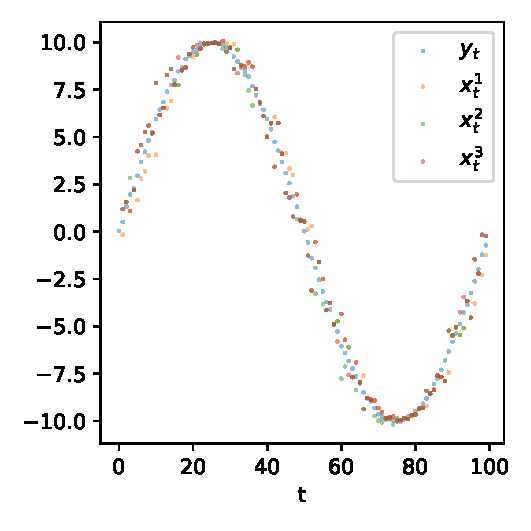
\includegraphics{plots/simulation_same_rmse_mae/time_series.pdf}
%   \caption{Realisation of Simulation~\ref{sec:simulation_rmse_mae} with $T = 100$, $\sigma_y=0.1$, $a = 10$, $p_2 = 0.8$, and $p_3 = (0.9, 0.5)$}
%   \label{fig:simulation_rmse_mae_ts}
% \end{figure}

% \begin{figure}
%   \centering
%   \begin{subfigure}{.32\textwidth}
%   	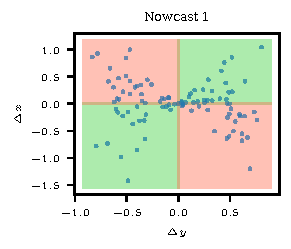
\includegraphics{plots/simulation_same_rmse_mae/4q_plot_1}
%   \end{subfigure}
%   \begin{subfigure}{.32\textwidth}
%   	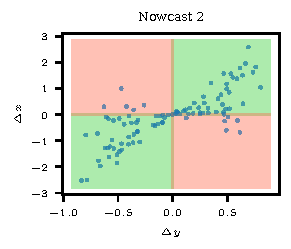
\includegraphics{plots/simulation_same_rmse_mae/4q_plot_2}
%   \end{subfigure}
%     \begin{subfigure}{.32\textwidth}
%   	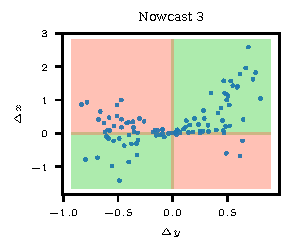
\includegraphics{plots/simulation_same_rmse_mae/4q_plot_3}
%   \end{subfigure}
%   \caption{4Q-Plot for Simulation~\ref{sec:simulation_rmse_mae} with $T = 100$, $\sigma_y=0.1$, $a = 10$, $p_2 = 0.8$, and $p_3 = (0.9, 0.5)$.}
%   \label{fig:simulation_rmse_mae_4q}
% \end{figure}

% \todo[inline]{Weiteres Beispiel für viele richtigen Punkte sehr nah an den Entscheidungsgrenzen.}
% \subsection{Simulation: Bootstrap}

% Simulation setup:

% \begin{itemize}
%   \item $T = 10,000$
%   \item $\ydiff_t \sim N(0, 1)$ 
%   \item $\xdiff_t^{1, k} = b_t  \ydiff_t, b_t \sim \SBer(k)$ (symmetric Bernoulli)
% \end{itemize}
% \unsure[inline]{(or both + random (non-systematic) noise?)}

% Analysis:
% \begin{itemize}
% \item Do for $l = 1, \dots, 100$:
% \begin{itemize}
%   \item Sample $\ydiff, \xdiff$
%   \item Compute bootstrap confidence intervals $(b_{low}, b_{up})_l$ using $B = 10,000$
% \end{itemize}
%   \item Visualize all intervals with real value (confidence interval should cover real value in $\alpha$ cases)
% \end{itemize}



\subsection{Effect of increasing sample size?}

\section{Application on disease and economic data}

\subsection{Nowcasts for the COVID infections in Germany}

\begin{itemize}
  \item Describe QoI and Nowcasts; which nowcasts do we consider? Which data is available when?
  \item Plot data
\end{itemize}

\subsection{Nowcasting of GDP}

\section{Conclusion}
\medskip
\printbibliography

\appendix
% \section{Illustrative examples for probabilistic measures}

% \begin{figure}
%     \centering
%     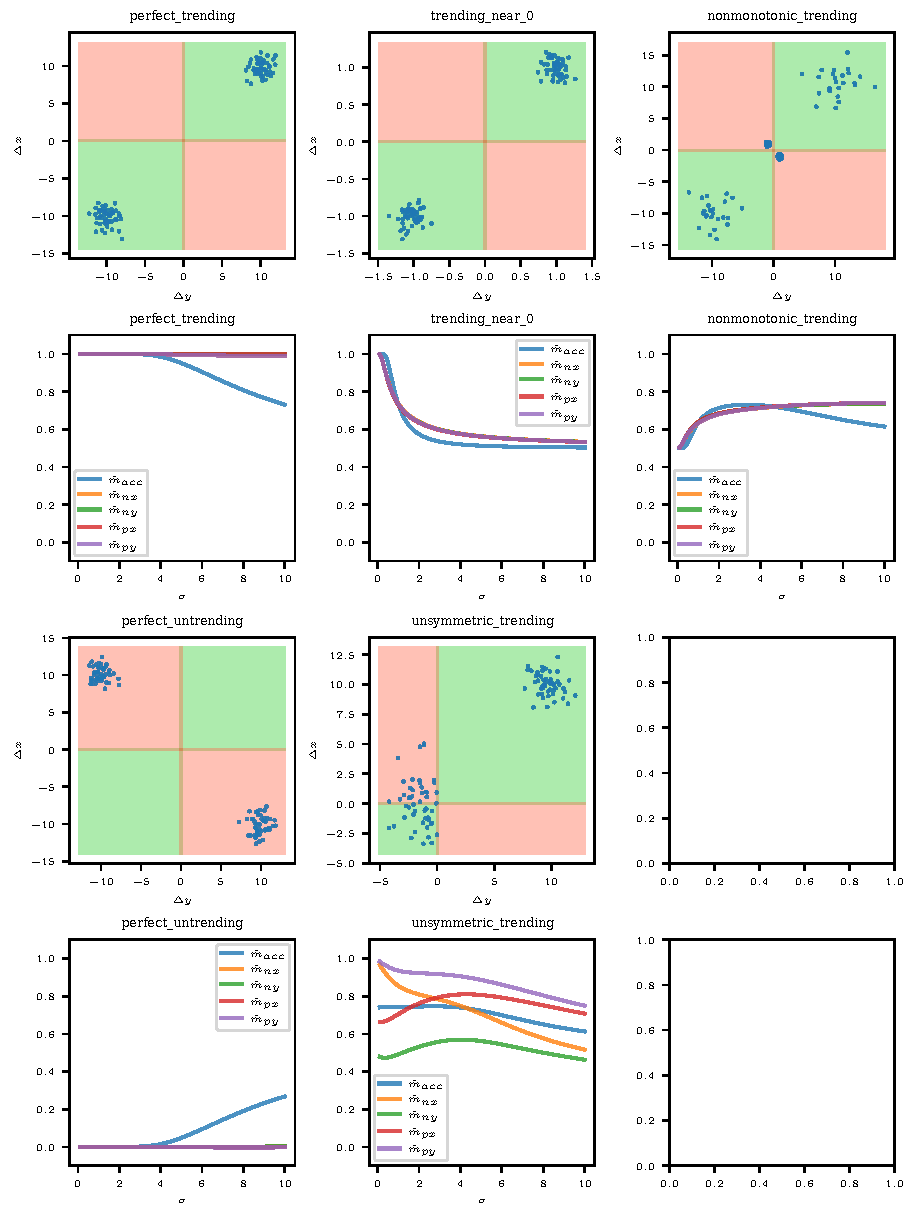
\includegraphics{plots/illustrative_examples/plots_4q_and_mtilde.pdf}
%     \caption{Various examplary courses of the measures $\tilde{m}$ for different configurations of $\ydiff$ and $\xdiff$}
%     \label{fig:example_mtilde}
% \end{figure}

\end{document} 